\documentclass{article}


\usepackage[latin1]{inputenc}
\usepackage{hyperref}
\usepackage{graphicx}
\usepackage{amsmath, amssymb}
\usepackage{stmaryrd}

%%%%%%%%%%%%%%%% Lengths %%%%%%%%%%%%%%%%
\setlength{\textwidth}{15.5cm}
\setlength{\evensidemargin}{0.5cm}
\setlength{\oddsidemargin}{0.5cm}

%%%%%%%%%%%%%%%% Variables %%%%%%%%%%%%%%%%
\def\projet{5}
\def\titre{Interpolation and integration methods / Cubic splines and surface interpolation}
\def\groupe{2}
\def\equipe{2}
\def\responsible{chelou001}
\def\secretary{desparbes}
\def\others{lgrelet, ndehaiesdit, tagry}

\begin{document}

%%%%%%%%%%%%%%%% Header %%%%%%%%%%%%%%%%
\noindent\begin{minipage}{0.98\textwidth}
  \vskip 0mm
  \noindent
  { \begin{tabular}{p{7.5cm}}
      {\bfseries \sffamily
        Project \projet} \\
      {\itshape \titre}
    \end{tabular}}
  \hfill
  \fbox{\begin{tabular}{l}
      {~\hfill \bfseries \sffamily Group \groupe\ - Team \equipe
        \hfill~} \\[2mm]
      Responsible : \responsible \\
      Secretary : \secretary \\
      Coders : \others
    \end{tabular}}
  \vskip 4mm ~

  ~~~\parbox{0.95\textwidth}{\small \textit{Abstract:} \sffamily This project implements a (somewhat basic) model to represent the air flow around an airfoil, i.e. the cross section of an aircraft's wing. The goal consists in obtaining a pressure map above and below the wing, so as to approximate the wing's lift, i.e. its ability to sustain the plane in the air. This is to be done in two steps: first, refine the airfoil into a sufficiently smooth curve, then compute the pressure map using integration methods. }
  \vskip 1mm ~
\end{minipage}

%%%%%%%%%%%%%%%% Main part %%%%%%%%%%%%%%%%
\section{Cubic spline interpolation method}

To obtain an accurate model of air flow, some mathematic tools are needed. First of all, it is necessary to implement an interpolation method. It consists in computing an approximation of a function, based on a finite sample of values taken by this function in known points. In this project, the cubic spline method is chosen: here, the approximation between two consecutive points is a third degree polynom. The continuity of two consecutive polynoms, their derivates and their second derivate is kept to guanrantee the global cohesion of the solution. An interresting choice to compute the cubic spline method is to calculate the second derivate first, and then to deduce the interpolation function itself. The algorithm used in this project is based on an \href{http://www.labri.fr/perso/fpierre/documents_enligne/c3-3.ps}{already-existing code} written in C we adapted to Python. Here is an example of the second derivate of cosinus on $[0, \pi]$ obtained with this algorithm:

\begin{figure}[h]
  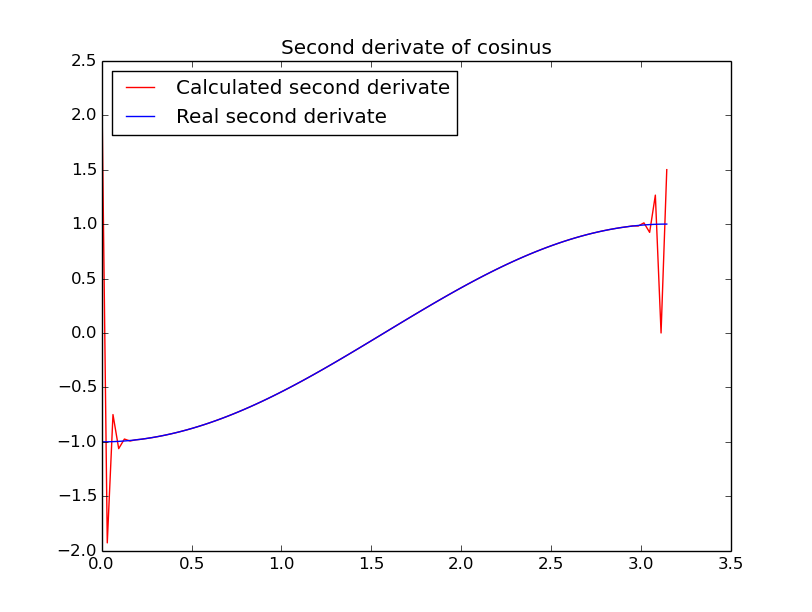
\includegraphics[width=12cm]{cosinus_second_derivate}
\end{figure}

This graph is a comparison between the curve obtained with this algorithm and the real representation of the second derivate of cosinus, which is

\begin{equation}
\begin{array}{ccccl}
\frac{d^2 cos}{dx^2} & : & [0, \pi] & \to & \mathbb{R} \\
 & & x & \mapsto & -cos(x)
\end{array}
\end{equation}

The two curves are similar, but obviously, there are disturbances on each extremity of the computed one. It means that this algorithm sometimes doesn't give a satisfying result for the extreme side values of the considerated interval. This fact will be important for the interpretation of the following results.\\\\

Now that a good approximation of the second derivate of the function is calculated, it is clearly possible to compute the function itself. This is an example of an cubic spline interpolation of cosinus on $[0, \pi]$ :

\begin{figure}[h]
  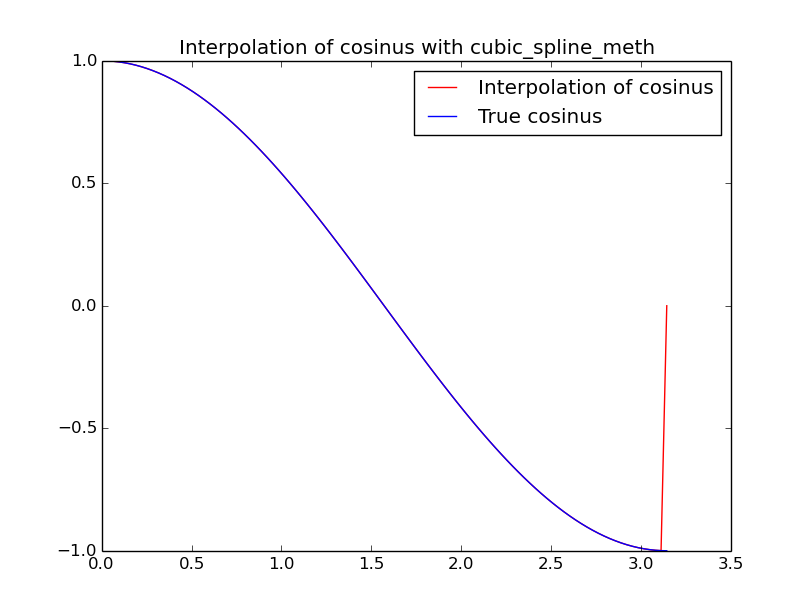
\includegraphics[width=12cm]{cosinus_interpolation}
\end{figure}

Once again, the computed curve follows the real cosinus curve, but diverges at the end of the interval. This might be due to the bad accuracy of the second derivate algorithm for the last values of the interval.

\section{Integration methods}
In order to map the pressure arround the wing, an integration algorithm is needed. Here are implemented three different methods: the classical rectangle method, the Simpson's method and the midpoint method.

\subsection{Rectangle integration method}
With this method, calculating the integral of a continuous function $f$ between $a$ and $b$ consists in summing the surfaces of $n$ rectangles defined by:
\begin{itemize}
\item the width of each rectangle is $\frac{b - a}{n}$
\item the height of rectangle $i \in \llbracket 0, n - 1 \rrbracket$ is $f(a + i\frac{b - a}{n})$ for the left rectangle method
\item the height of rectangle $i \in \llbracket 1, n \rrbracket$ is $f(a + i\frac{b - a}{n})$ for the right rectangle method
\end{itemize}
Left and right methods are similar: they converge to the same value at the same speed.

\subsection{Simpson's integration method}
Simpson's method consists in summing the integrals of $n$ quadratic polynoms. Each polynom is a Lagrangian interpolation of the function on three consecutive points.
As a consequence, for each polynom $P_i$ with $i \in \llbracket 0, n - 2 \rrbracket$, $P_i(a + i \frac{b-a}{2n}) = P_{i+1}(a + i \frac{b-a}{2n})$. Once the interpolations are made, it is easy to calculate their integral (polynom of degree 2), and then to sum them. Because there are twice as points as quadratic polynoms, it is better to use an even number of points, or the last point, which is associated with no polynom, will degrade the accuracy of the algorithm. This phenomenom is observable on the graphs below.

\subsection{Midpoint integration method}
This method is similar to the classical rectangle method, except that instead of aligning the rectangles to the left or to the right, each rectangle is centered on the considered point. It is predictable that it doesn't accelerate the convergence, but each iteration of this method is generaly more accurate than the rectangular one.

\subsection{Comparison between the different methods}

A good way to compare these different algorithms is to show the value of the integral calculated with each method with the same number of iterations. For exemple, in the test file is computed the integral between $0$ and $\frac{\pi}{2}$ of cosinus, which is 1. After 100 iterations, the results are:
\begin{itemize}
\item 1.00783341987 for the rectangle method
\item 1.00000000034 for the Simpson's method
\item 1.00001028091 for the middle point method
\end{itemize}
This means that, based on this criteria, the best algorithm is Simpson's method, then comes the middle point method and finally the rectangle method.
\newpage

It is also possible to display a graph representing the integral obtained in function of the number of iterations for each algorithm:

\begin{figure}[h]
  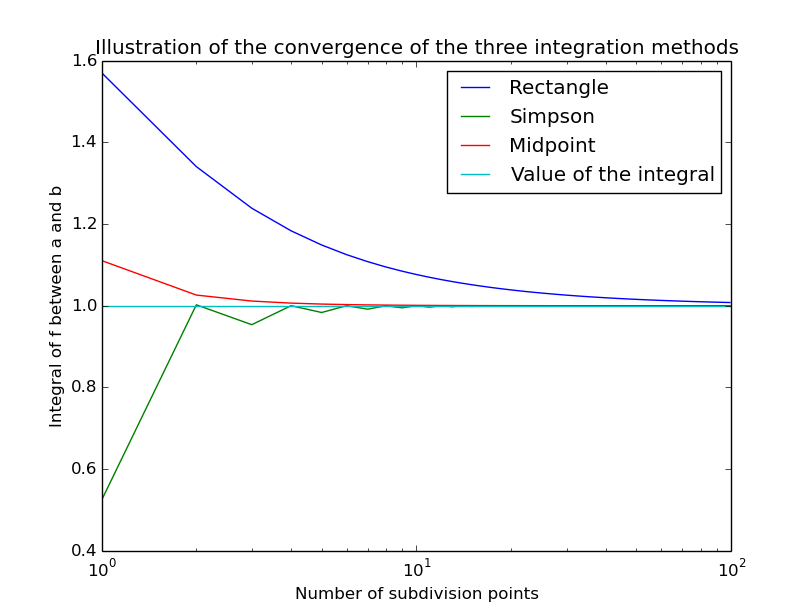
\includegraphics[width=12cm]{cosinus_integration}
\end{figure}

On this example, it is clear that the rectangle method is the less efficient algorithm of the three. But as explained before, the Simpson's method alternates between a really accurate approximation for even iterations and a poorer approximation for odd iterations. Globaly, Simpson's method stays the most efficient algorithm between the three, if an even number of iteration is chosen.

\section{Length of a portion of curve}

Once an interpolation and an integration tools are set, it is easy to calculate the length of a curve's portion of a function $f$, given the formula:
\begin{equation}
  L([a, b]) = \int^a_b{\sqrt{1 + (f'(x))^2} dx}
\end{equation} 
$f$ is interpolated with the cubic spline method, then derivated with a algorithm based on the manipulation of the coefficients of each polynom of the interpolation function. The function $s: u \mapsto \sqrt{1 + u^2}$ is then applicated. After the interpolation of $s$, it is finally possible to calculate its integral.

\section{Modelization of the airflow arround a wing}

All the mathematic tools are now set, it is possible to use it in order to modelize the airflow arround the wing of a plane. After extracting the airfoil from a file with discrete values, it is easy to get an interpolation of the intrados and of the extrados. A simple model of the airflow on the extrados can be computed using this formula:
\begin{equation}
\forall \lambda \in [0,1]: f_{\lambda}(x) = (1-\lambda)f(x) + 3\lambda h_{max}
\end{equation}
with $f: D \to \mathbb{R}$ the function which associates the ordinate of the extrados of the aifoil to each abscissa and $h_{max} = max_{x \in D}(f(x))$. A similar formula is used for the intrados, replacing $h_{max}$ by $h_{min}$ and $f$ by $g$, the function which associates the ordinates of the intrados. Here is an example of the airflow arround the airfoil of a Boeing:

\begin{figure}[h]
  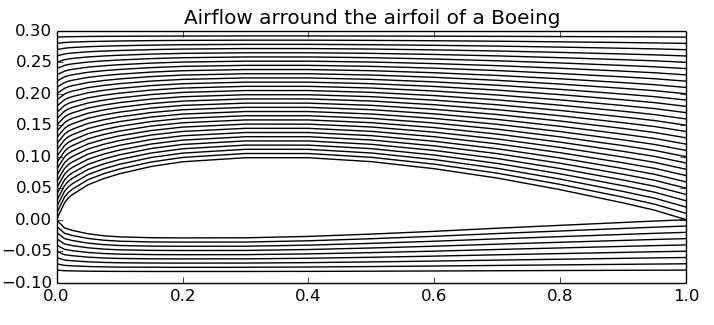
\includegraphics[width=12cm]{boeing_airflow}
\end{figure}

It is noticeable that the path of the airflow in contact with the extrados is longer than the path of the airflow in contact with the intrados. A particule which is in $x = 0$ at $t = 0$ will arrive at the same date $t_{end}$ at $x = x_{end}$ independently of $y$, that is to say the particules on the extrados are travelling faster than those on the intrados. With the Bernouilli's law, which says that a the dynamic pressure of a fluid is proportionnal to the square of its speed, it is possible to map the pressure arround the airfoil.





\end{document}
